\subsection{アナログ入力そうちを使ってみよう}
デジタル入力そうちをHSPで使ってみましょう。GPIO24にボタン(\#103)をつけてください。HSPスクリプトエディタで/home/pi/ome/05/digin.hspを開いて実行してみましょう。\\
\begin{figure}[H]
    \centering
    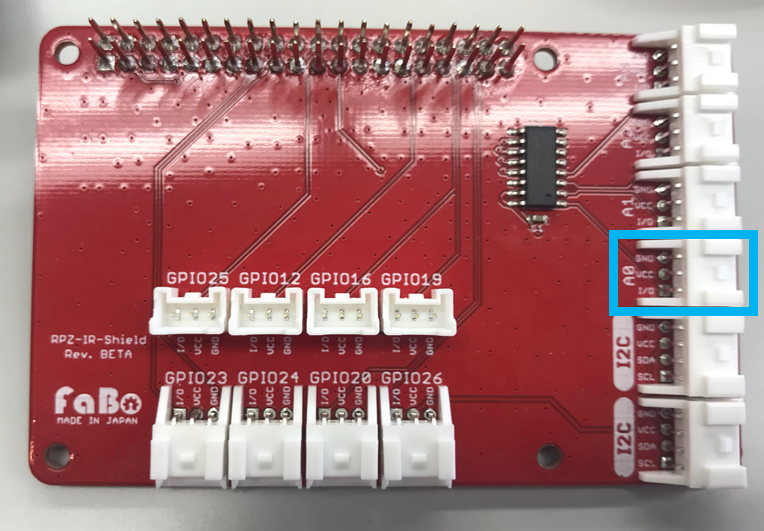
\includegraphics[scale=0.8]{images/chap05/text05-img030.png}
    \caption{アナログ入力A0}
\end{figure}

\begin{lstlisting}[caption=anain.hsp,label=anain.hsp]
#include "hsp3dish.as"
#include "rpz-gpio.as"

spiopen 0	<#blue#;SPIチャンネルを開く#>

*main
	data = spiget(0,0)	<#blue#;SPIを使ってデータを受け取る#>
	res = "結果 : "+data+"\n"

	redraw 0
	pos 20,20
	font "",30
	mes res
	redraw 1

	wait 10
	goto *main

spiclose 0	<#blue#;SPIチャンネルを閉じる#>
\end{lstlisting}

anain.hspはアナログ入力そうち用のプログラムです。アナログ入力にはA0,A1,A2,A3のピンを使います。感圧センサー、ボリューム、距離センサー、照度センサーを使うことができます。

アナログ入力そうちから入力を受け取るときにSPI(Serial Peripheral Interface)という方法を使っています。\code{spiopen 0}命令を使ってラズベリーパイとアナログ入力そうちをつなげます。\code{spiclose 0}命令を使ってラズベリーパイとアナログ入力そうちのつながりを切ります。

アナログ入力は\code{spiget(ピン番号,0)}で値を受け取ります。ピン番号はブリックがつながっている番号です。入力される値は0~1023までの数字になります。詳しいアナログ入力そうちの使い方は\pageref{analog_in}ページから見てみましょう。\\

\begin{tcolorbox}[title=\useOmetoi]
\begin{enumerate}
\item 感圧センサー(\#106)をA0につなげて上記のanain.hspを実行してみましょう。感圧センサーにさわる強さによって、画面の数字が変わります。
\end{enumerate}
\end{tcolorbox}
\begin{tcolorbox}[title=\useOmetoi]
\begin{enumerate}
\item ボリューム(\#104)をA0につなげてanain.hspを実行してみましょう。ボリュームを動かすと、画面の数字が変わります。
\end{enumerate}
\end{tcolorbox}
\begin{tcolorbox}[title=\useOmetoi]
\begin{enumerate}
\item 照度センサー(\#109)をA0につなげてanain.hspを実行してみましょう。明るさによって、画面の数字が変わります。
\end{enumerate}
\end{tcolorbox}
\begin{tcolorbox}[title=\useOmetoi]
\begin{enumerate}
\item \code{spiget(0,0)}を\code{spiget(1,0)}に変えましょう。A1にアナログ入力そうちをつなぎましょう。anain.hspを実行してみましょう。
\end{enumerate}
\end{tcolorbox}